\section{\sloppy Comparing Linux-Based and Real-Time Operating Systems}
% \section*{\sloppy Comparing Linux-Based and Real-Time Operating Systems}
% \addcontentsline{toc}{section}{Comparing Linux-Based and Real-Time Operating Systems}
% Remove header text
\markboth{}{}
    RTOSs provide safety and predictability to the system they support.
    The ability to meet deadlines when responding to external events is
        necessary for hard real-time systems and crucial for soft ones.
    The price for this assurance is increased complexity, cost, and development
        time.
    Alternatively, Linux-based operating systems feature a suite of tools for
        handling soft real-time requirements.
    And, by virtue of the Linux kernel being open source, it can be extended to
        further meet real-time requirements by developers with expert Linux
        knowledge.
    Deciding whether to switch from a Linux distribution to a RTOS involves
        analyzing the benefits of a RTOS and balancing them with their
        associated costs.
    These benefits and tradeoffs between will be discussed here.
    But first, it must be acknowledged that there is a high degree of overlap
        between the two, especially regarding soft real-time systems.

        \subsection{The Overlap Between Linux-Based and Real-Time Operating Systems}
        % \subsection*{The Overlap Between Linux-Based and Real-Time Operating Systems}
        % \addcontentsline{toc}{subsection}{The Overlap Between Linux-Based and Real-Time Operating Systems}
        % Remove header text
        \markboth{}{}
            When utilizing Linux for real-time systems, there are generally two
                options.
            The first is to use the real-time capabilities built into the Linux
                kernel.
            One such capability is a patch to the kernel that makes it fully
                preemptible.
            The second option is to use a real-time framework for the Linux
                kernel.
            Three such frameworks are discussed, all of which function by adding
                a \textit{co-kernel} in a addition to the Linux kernel.

            \subsubsection{The Fully Preemptible Linux Kernel}
            % \subsubsection*{The Fully Preemptible Linux Kernel}
            % \addcontentsline{toc}{subsubsection}{The Fully Preemptible Linux Kernel}
                The real-time features of the Linux kernel revolve around
                    \textit{preemption}---pausing a running process to run a
                    higher-priority process instead.
                In user-mode, any process can be preempted, transferring control
                    to the kernel for scheduling \cite{ubuntu-real-time-part2}.
                The preemption strategy for kernel mode is where the potential
                    for real-time Linux lies.
                Mainline Linux (the vanilla version of the Linux kernel not
                    associated with any specific distribution) offers three
                    preemption strategies for the kernel:
                \begin{itemize}
                    \item
                        \textbf{PREEMPT\_NONE} forbids preemption when in
                            kernel mode; system call returns and interrupts are
                            the only preemption points
                            \cite{linux-preemption-models}.
                    \item
                        \textbf{PREEMPT\_VOLUNTARY} allows low-priority
                            processes to voluntarily preempt themselves when
                            executing a system call in kernel mode
                            \cite{ubuntu-real-time-part3}.
                    \item
                        \textbf{PREEMPT} makes all kernel code preemptible,
                        except for critical sections
                        \cite{linux-preemption-models}.
                \end{itemize}

                The fully preemptible kernel (the \textbf{PREEMPT\_RT} patch)
                    takes preemption further.
                This patch aimed to give Linux even more real-time capabilities.
                Although not part of mainline Linux, this patch is backed by the
                    Linux Foundation and is in use for real-time systems
                    \cite{rt-linux-riscv}.
                This preemption strategy further increases the number of
                    preemption points in kernel code and uses more real-time
                    data structures when handling interrupts and threads
                    \cite{linux-preemption-models}.

                The fully preemptible Linux kernel can be utilized in
                    high-performance computing and embedded industrial
                    environments.
                For complex real-time systems this kernel configuration provides
                    real-time capabilities within the familiarity of a
                    Linux-based operating system.
                The primary caveat is that there is no formal guarantee of worst
                    case execution times, and thus cannot be used for
                    safety-critical real-time systems \cite{preempt-rt-survey}.

            \subsubsection{Real-Time Linux Frameworks}
            % \subsubsection*{Real-Time Linux Frameworks}
            % \addcontentsline{toc}{subsubsection}{Real-Time Linux Frameworks}
            % Remove header text
            \markboth{}{}
                Other than the fully preemptible Linux kernel, the most common
                    approach to adapting the Linux kernel to real-time
                    environments involves using a real-time framework that adds
                    a co-kernel to the Linux kernel.
                The idea is to have the co-kernel working as a layer between the
                    hardware and the Linux kernel.
                The co-kernel is responsible for catching hardware interrupts,
                    scheduling them as either real-time tasks or Linux tasks,
                    and guaranteeing that real-time tasks meet their deadline.
                Leftover CPU time is given back to the Linux kernel
                    \cite{preempt-rt-survey}.

                The most common open-source implementations of a real-time
                    co-kernel Linux framework are RTLinux, Xenomai, and the Real
                    Time Application Interface for Linux (RTAI).

                \begin{itemize}
                    \item
                        \textbf{RTLinux} runs the Linux kernel as a
                            fully-preemptible process \cite{preempt-rt-survey}.
                        It then intercepts all hardware interrupts and schedules
                            tasks.
                        Shown in \fig{rtlinux_structure}, hardware interrupts
                            not related to real-time events are passed to the
                            Linux kernel as software interrupts, whereas
                            real-time event interrupts are handled by the
                            appropriate real-time interrupt service routines
                            \cite{rt-linux-getting-started}.
                        \begin{figure}[H]
                            \centering
                            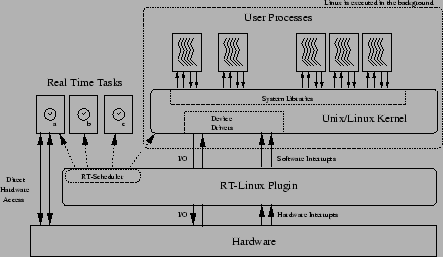
\includegraphics
                                [width=0.7\textwidth]
                                {images/rtlinux_structure.png}
                            \caption
                                [Structure of RTLinux]
                                {Structure of RTLinux \cite{rt-linux-getting-started}.}
                            \label{fig:rtlinux_structure}
                        \end{figure}
                    \item
                        \textbf{Xenomai} works by supplementing the Linux kernel
                            with a real-time kernel running side-by-side with
                            it \cite{xenomai-overview}.
                        The real-time core deals with all time-critical
                            tasks and has a higher priority than the Linux
                            kernel.
                        The Xenomai kernel and the Linux kernel communicate via
                            the
                            \textit{Adaptive Domain Environment for Operating System (ADEOS)},
                            which separate domains for both kernels
                            \cite{preempt-rt-survey}.
                        This is shown in \fig{xenomai_structure}.
                        \begin{figure}[H]
                            \centering
                            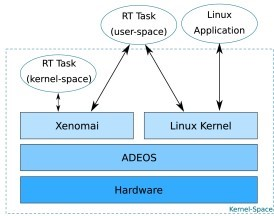
\includegraphics
                                [width=0.5\textwidth]
                                {images/xenomai_structure.jpg}
                            \caption
                                [Structure of Xenomai]
                                {Structure of Xenomai \cite{preempt-rt-survey}.}
                            \label{fig:xenomai_structure}
                        \end{figure}
                    \item
                        \textbf{RTAI} uses a hardware abstraction layer (RTHAL)
                            to get information from Linux and dispatch
                            interrupts \cite{xenomai-overview}.
                        This is displayed in \fig{rtai_structure}.
                        It has few dependencies to Linux, making it easy to
                            switch between versions of the Linux kernel
                            \cite{xenomai-overview}.
                        \begin{figure}[H]
                            \centering
                            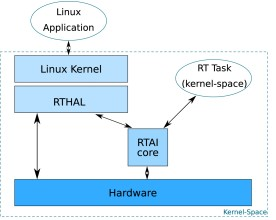
\includegraphics
                                [width=0.5\textwidth]
                                {images/rtai_structure.jpg}
                            \caption
                                [Structure of RTAI]
                                {Structure of RTAI \cite{preempt-rt-survey}.}
                            \label{fig:rtai_structure}
                        \end{figure}
                \end{itemize}

            \subsubsection{Choosing Between the Preemptible Kernel and Real-Time Frameworks}
            % \subsubsection*{Choosing Between Preemptible Kernel and Real-Time Frameworks}
            % \addcontentsline{toc}{subsubsection}{Choosing Between Preemptible Kernel and Real-Time Frameworks}
            % Remove header text
            \markboth{}{}
                The fully preemptible Linux kernel and real-time Linux kernel
                    frameworks both add real-time capabilities to the Linux
                    kernel.
                The fully preemptible kernel achieves this by allowing the
                    kernel to be preempted in kernel mode and utilizing
                    real-time data structures \cite{linux-preemption-models}.
                However, these modifications are not enough to accommodate the
                    needs of a hard real-time system \cite{preempt-rt-survey}.
                At its core, the PREEMPT\_RT patch is still the Linux kernel,
                    offering no guarantees on worst case execution time
                    \cite{preempt-rt-survey}.
                This approach should only be taken for soft real-time systems.
                In this use case, the most important advantage of using the
                    fully preemptible Linux kernel is the cost and speed of
                    development.
                PREEMPT\_RT Linux does not differ much from mainline Linux.
                This allows the wealth of code for drivers and libraries in
                    Linux to be reused---although they may need to be adapted to
                    fit real-time needs.
                Further, many software engineers are competent with Linux and
                    can handle developing with the PREEMPT\_RT patch
                    \cite{preempt-rt-survey}.

                When tighter deadlines are required, a co-kernel Linux framework
                    can be used.
                These frameworks do have the ability to handle hard real-time
                    requirements \cite{preempt-rt-survey}.
                The cost of this functionality is development time and
                    complexity.
                Co-kernel approaches require modifications of the Linux kernel
                    code, none of which are fully backed by the
                    Linux community.
                This also introduces a dependency on the specific Linux kernel
                    version being modified, often being an older version
                    \cite{preempt-rt-survey}.
                The complex interaction between the two kernels introduces a
                    level of complexity that needs to be handled by skilled
                    real-time developers, increasing development efforts
                    \cite{preempt-rt-survey}.
                As a result, real-time Linux frameworks should be used only when
                    necessary, preferring the fully preemptible kernel when
                    timing requirements allow it.

        % Remove header text
        \markboth{}{}
        \subsection{Non-Linux-Based Real Time Operating Systems}
        % \subsection*{Non-Linux-Based Real Time Operating Systems}
        % \addcontentsline{toc}{subsection}{Non-Linux-Based Real Time Operating Systems}
        % Remove header text
        \markboth{}{}
            There are many RTOSs that are not associated with the Linux kernel.
            Some of these operating systems are open source, others are
                commercially available.
            They have different use cases when compared with each other, and
                when compared with Linux-based alternatives.
            These use cases will be presented here, along with examples of
                non-Linux RTOSs.

            \subsubsection{Advantages and Disadvantages of Non-Linux-Based Real-Time Operating Systems}
            % \subsubsection*{Advantages and Disadvantages of Non-Linux-Based Real-Time Operating Systems}
            % \addcontentsline{toc}{subsubsection}{Advantages and Disadvantages of Non-Linux-Based Real-Time Operating Systems}
            % Remove header text
            \markboth{}{}
                The main advantage of using the Linux kernel for real time
                    systems is the ease of development.
                Many software engineers are familiar with Linux and can quickly
                    learn how to use the real-time capabilities of the kernel.
                Soft real-time systems can make use of the fully preemptible
                    kernel, while hard real-time systems require a framework
                    that modifies the kernel.
                However, real-time Linux-based operating systems, whether it is
                    the fully preemptible kernel or a real-time kernel
                    framework, require the memory space and processing power to
                    run a full Linux operating system.
                This is a luxury that many embedded systems simply do not have
                    \cite{rtos-overview}.
                Apart from very large real-time systems, another solution is
                    needed.
